\documentclass[11pt]{article}

\usepackage[utf8]{inputenc}
\usepackage[margin=2cm]{geometry} 
\usepackage{hyperref}
\usepackage{graphicx}
\usepackage{float}
\usepackage{caption}
\usepackage{longtable}
\usepackage{minted}
\usepackage{appendix}
\usepackage{xcolor}
\usepackage{subfig}
\usepackage{bookmark}
\usepackage{array}
\usepackage{multirow}

\setlength{\parskip}{1em}
\setlength{\parindent}{0pt}

\title{Data Mining \& ML}
\author{Group 4\\Lewis Wilson, Sam Fay-Hunt, Kamil Szymczak, Chun Man }
\date{November 2020}

\begin{document}

\maketitle

\pagebreak

%TABLE OF CONTENTS
\tableofcontents
\thispagestyle{empty}
\pagebreak
\setcounter{page}{1}

\pagebreak

\section{File management, data pre-processing, transformation and selection} 
\subsection{File Management}

To facilitate collaboration and reduce repetition we developed a Scripts module (See Figure~\ref{tab:moduleTable}) containing the majority of our code for this coursework. These functions provide utility for loading data, pre-processing data, building models and other convenience tasks. We annotated all functions within the Scripts module with docstrings, and compiled them with Sphinx, a final version of the documentation can be found under '\emph{docs.rar}' in the project root folder.
\par
We used Jupyter notebooks for all the tasks, primarily as a testing workspace and a medium to present our final work.

\subsection{Data pre-processing}\label{sec:transSel}
\subsubsection{Data transformation}
\textbf{\underline{Downsampling}}\\
We used local-mean downscaling (\emph{Scripts/downsampling.py}) to try and expose low-level features
(Appendix~\ref{fig:downsampleExample}). We frequently used downscaling throughout the project to reduce the image resolution by averaging 4 pixels into 1. 
We also used rescaling with aliasing to reduce the image to 12x12 pixels, to aid in visualising patterns in the pixel greyscale values (Appendix~\ref{12x12Scatter}~\&~\ref{AvColDSvAvRowDS}).
\par

\textbf{\underline{Binning}}\\
By implementing equal width binning we were able to greatly reduce the cardinality of the greyscale values from 256 to 8. 
This helped offload a considerable amount of computation when calculating the edges in the complex Bayes Networks, and offered a small accuracy uplift for the Naive Bayes classifier (see Section~\ref{sec:NaiveBayse}).

\subsubsection{Data selection}
\textbf{\underline{Balancing the class distribution}}\\
Having observed frequent issues with overfitting due to a substantial imbalance in the class distributions (particularly with the binary classification labels) we utilised the sample method from the Pandas library along side the random\_state argument to produce replicable datasets with a balanced number of each distinct class.

\textbf{\underline{Sampling data}}\\
We primarily used the train\_test\_split function from the SKLearn library because it provides excellent utility for splitting apart the data with parameters to aid in discretizing, replicating, and resizing the data.
We also made use of Pandas and Numpy shuffle methods when most convenient.

\textbf{\underline{Pixel Selection}}\\
(Figure ~\ref{train_2304})
We produced pairwise correlations between each pixels value and the class label, then using this data we produced an ordered list of pixel indices for each label file. We used this data to produce heatmaps showing the importance of each pixel (See Appendix~\ref{Heatmaps}), where the darkest pixels are deemed the most important for prediction and the lightest the least.
We used the pixel ordering data to build and score 2304 Naive Bayes classifiers for each class of labels, each plot on the x-axis is using all preceding pixels for classification see Figure in Appendix~\ref{train_2304}.

\section{Naive Bayesian Networks}\label{sec:NaiveBayse}
We used the SKLearn library's Naive Bayes modules to build the Naive Bayes classifiers, we built 88 classifiers so we could compare and test the various pre-processing configurations we had developed. 
First we plotted the accuracy of the different configurations in bar charts to provide a high-level perspective on the accuracy, and then we built confusion matrices gain detailed insight into how the classifier's performance varied.\\
\underline{Observations:}
\begin{enumerate}
    \item Using no pre-processing technique with Naive Bayes had a significant negative impact on the quality of the predictions.
    \item Downscaling on its own provides no observable benefit to the accuracy of Naive Bayes.
    \item Naive Bayes performs much better when it is only trained to perform binary classifications
    \item Naive Bayes has serious problems with overfitting when the distribution of classes in the dataset is poorly balanced.
    \item Under the right conditions Naive Bayes can make excellent predictions, we observed prediction accuracy as high as 88\% with our test data.
\end{enumerate}

\begin{figure}[H]
  \centering
  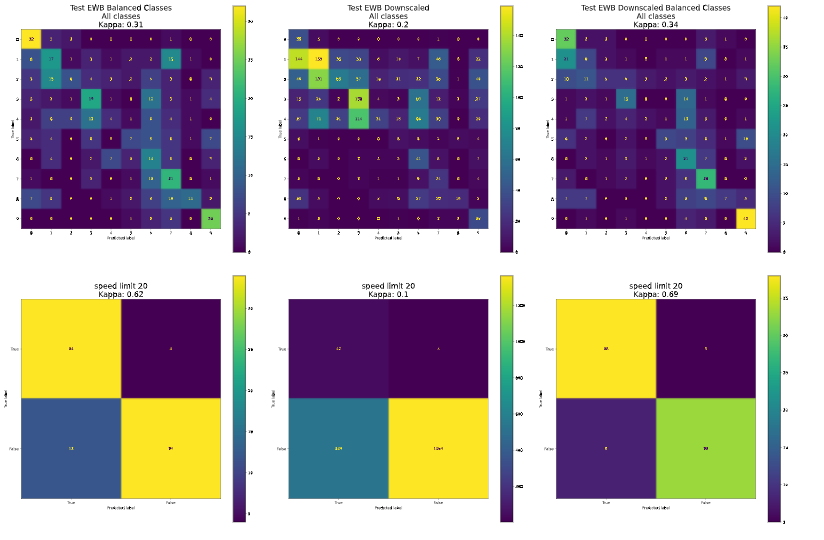
\includegraphics[width=0.9\textwidth]{Images/NaiveBayesEWBMatrices.png}
  \caption{Naive Bayes confusion matrix showing Equal Width Binning}
  \label{fig:NaiveBayesEWBConfMat}
\end{figure}
\section{Complex Bayes nets}
\subsection{Building Bayes Networks}
Bayes networks represent probabilistic directed acyclic graphs that define the relationships between conditional dependencies and random variables.
A naive Bayesian network can be represented in a Bayes network where the node representing the probability distribution of the class is the only parent of all other nodes and no other edges exist in the network. 
By adding additional edges (so long as the graph remains acyclic) we can represent causal relations between random variables.
\par
Using the pgmpy library we build Bayes Networks using K2 scoring and HillClimbing to infer the edges of the network. Next we calculated the model parameters using pgmpy's built-in MaximumLikelihoodEstimator, we also tried this with a BaysianEstimator using K2, and Dirichlet scoring mechanisms.
Attempting to build the network both ways gave us solid insights into the problems that would have to be solved to produce a Bayes Network.
We immediately encountered 2 computational complexity problems:
\begin{enumerate}
    \item Learning the optimal edges.
    \item Building all the model parameters
\end{enumerate}

We handled the first problem by discretizing the greyscale values using equal-width binning(see section~\ref{sec:transSel}) and using the data acquired from Task 5 to select a small number of columns to build the networks.
When using Weka to compute Bayesian networks we observed that Weka would perform extremely aggressive binning of the greyscale values often discretizing down to only 2 bins. This had a profound effect on the speed of learning the parameters and edges.

\subsection{Algorithms \& Data}


\subsection{Experimental Results}

\pagebreak

\section{Clustering}
\subsection{Identifying clusters}
We used the principle component analysis module from SKLearn to help plot the data as a scatter graph, this made it very clear we had a problem with how our data was distributed for clustering see Appendix~\ref{app:BadClustering}, this resulted in apparently meaningless clusters.
To resolve this we tried many permutations of selection techniques, discretizations, and transformations. 
We considered that the data must be clustering on features that were otherwise transparent to us, as a result we tried looking for patterns in the clustering behaviour such as looking at how the clustering algorithm grouped data by high-level features such as the shape of the signs.
We used KMeans clustering with the EM and Elkan algorithms...({\huge talk about this more})\\
Because we observed an issue with the desired class features not usefully dividing the data within the clustering dimensions we decided to use transfer learning to try and extract more useful feature vectors.
We used Keras to download VGG16 with weights trained on imagenet, by removing the (top) fully connected layers past the convolutional and pooling layers we were able to produce feature vectors for each image. Using these feature vectors with principle component analysis we were finally able to produce some clearly divided clusters for the binary classification labels. 
We also noted that this resulted in clusters that were split by the shape of the signs (triangle or square).   

\underline{Clustering by sign shape}
\par
(Figure ~\ref{TrianCircCluster1}) We clustered the data into 2 clusters with the hope that it would differentiate the sign's shape, one cluster for triangular the other for rectangular signs. One cluster got more images of a particular shape than the other but the difference was very small. 
(Figure ~\ref{TrianCircCluster2}) When clustering them again but now with each image only containing the 250 best pixels, the clusters did a better job as they contained a lot more signs of one shape than the other. Thus we reaffirmed our knowledge from the task 4 heatmap stating that apart from digits on signs the shape is the second most important feature. 

\huge Figures needed (see task 9)

\pagebreak
\appendix
\appendixpage
\addappheadtotoc
\begin{appendices}
\section{Appendix A}
\subsection{Module Table}\label{tab:moduleTable}
The following are located in the Scripts folder
\begin{table}[ht]
    \centering
    \begin{tabular}{|p{0.35\linewidth} | p{0.6\linewidth}|} 
      \hline
      \textbf{Module Name}  & \textbf{Description} \\ \hline
      helperfn.py & Provides functions to load and transform with all datasets required. \\ \hline
      downsample.py & Provides functions to downsample images  \\ \hline
      pixelFinder.py & Provides functions to find the most important pixels within a dataset of a chosen street sign. \\ \hline
      bayseNet.py & Provides functions used for getting a score for a model by testing all test data against labels. \\ \hline
      confusionMatrix.py & Provides functions for building and displaying confusion matrices as well as methods for calculating kappa values. \\ \hline
      plotScripts.py & Provides functions for plotting data into graphs \\ \hline
      wekaConversion.py & Provides functions to convert preprocessed data to be consumable by Weka\\ \hline
      clustering.py & Provides functions for getting information for clusters\\
      \hline
    \end{tabular}
\end{table}
% Appendix A.1

\subsection{Downsampling example}\label{fig:downsampleExample}
\begin{figure}[H]
    \centering
    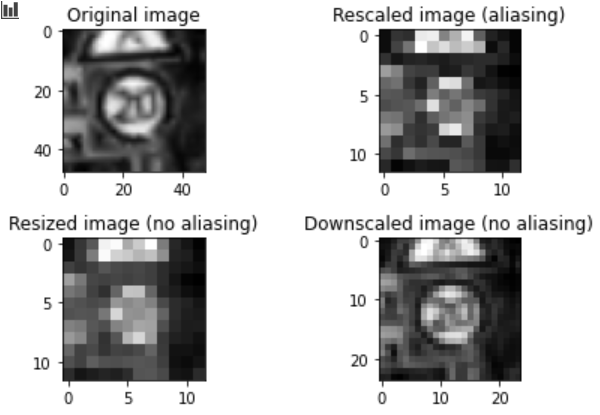
\includegraphics[width=0.9\textwidth]{Images/downsample_example.png}
\end{figure}

\newpage
\subsection{Heatmaps}\label{Heatmaps}
\begin{figure}[h!]
  \centering
  \begin{tabular}{ccc}
    \subfloat[20 mph \& 30 mph]{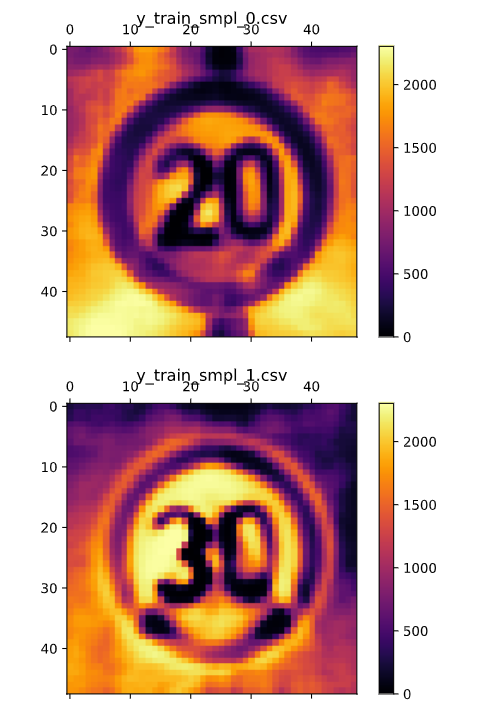
\includegraphics[width=0.3\textwidth]{images/heatmap.PNG}} &
    \subfloat[50 mph \& 60 mph]{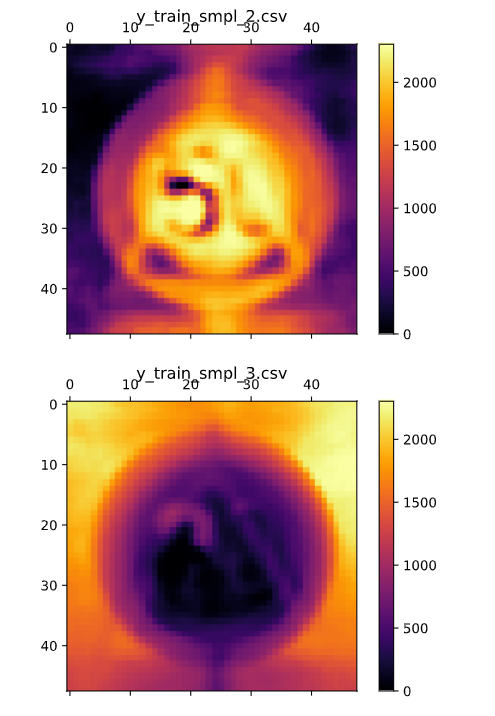
\includegraphics[width=0.3\textwidth]{images/heatmap2.PNG}} &
    \subfloat[70 mph \& left turn]{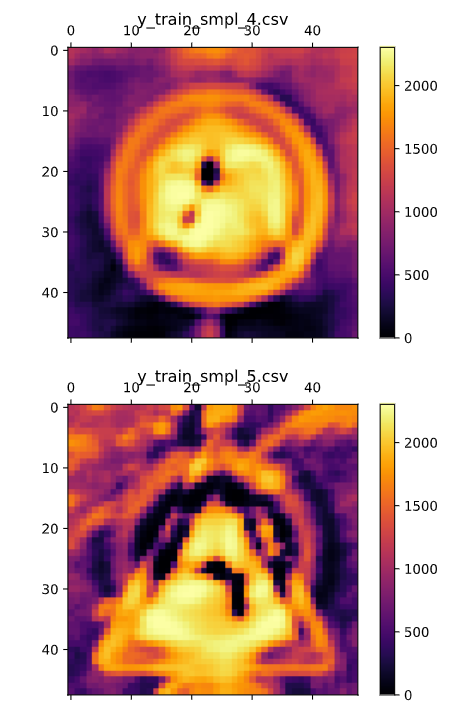
\includegraphics[width=0.3\textwidth]{images/heatmap3.PNG}} \\
    \subfloat[right turn \& beware pedestrian crossing]{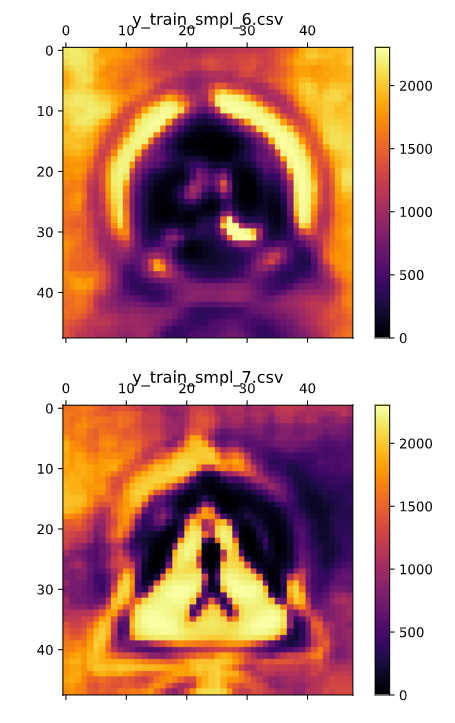
\includegraphics[width=0.3\textwidth]{images/heatmap4.PNG}} &
    \subfloat[beware children \& beware cycle route ahead]{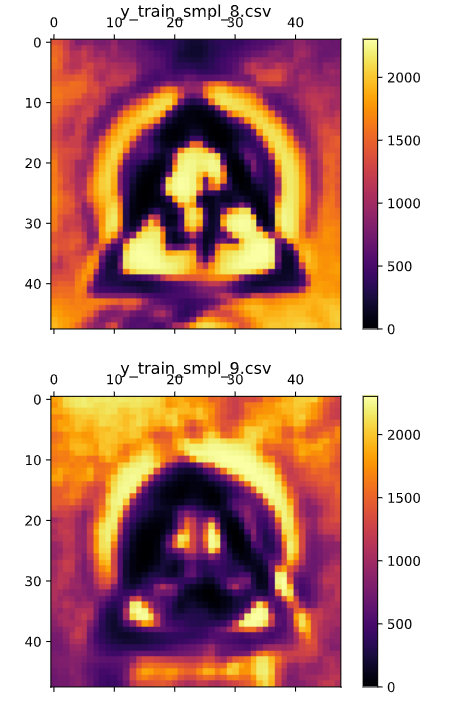
\includegraphics[width=0.3\textwidth]{images/heatmap5.PNG}} 
  \end{tabular}
\end{figure}

\newpage
\subsection{Accuracy of classifiers built using the first n pixels for each class}\label{train_2304}
\begin{figure}[h!]
  \centering
  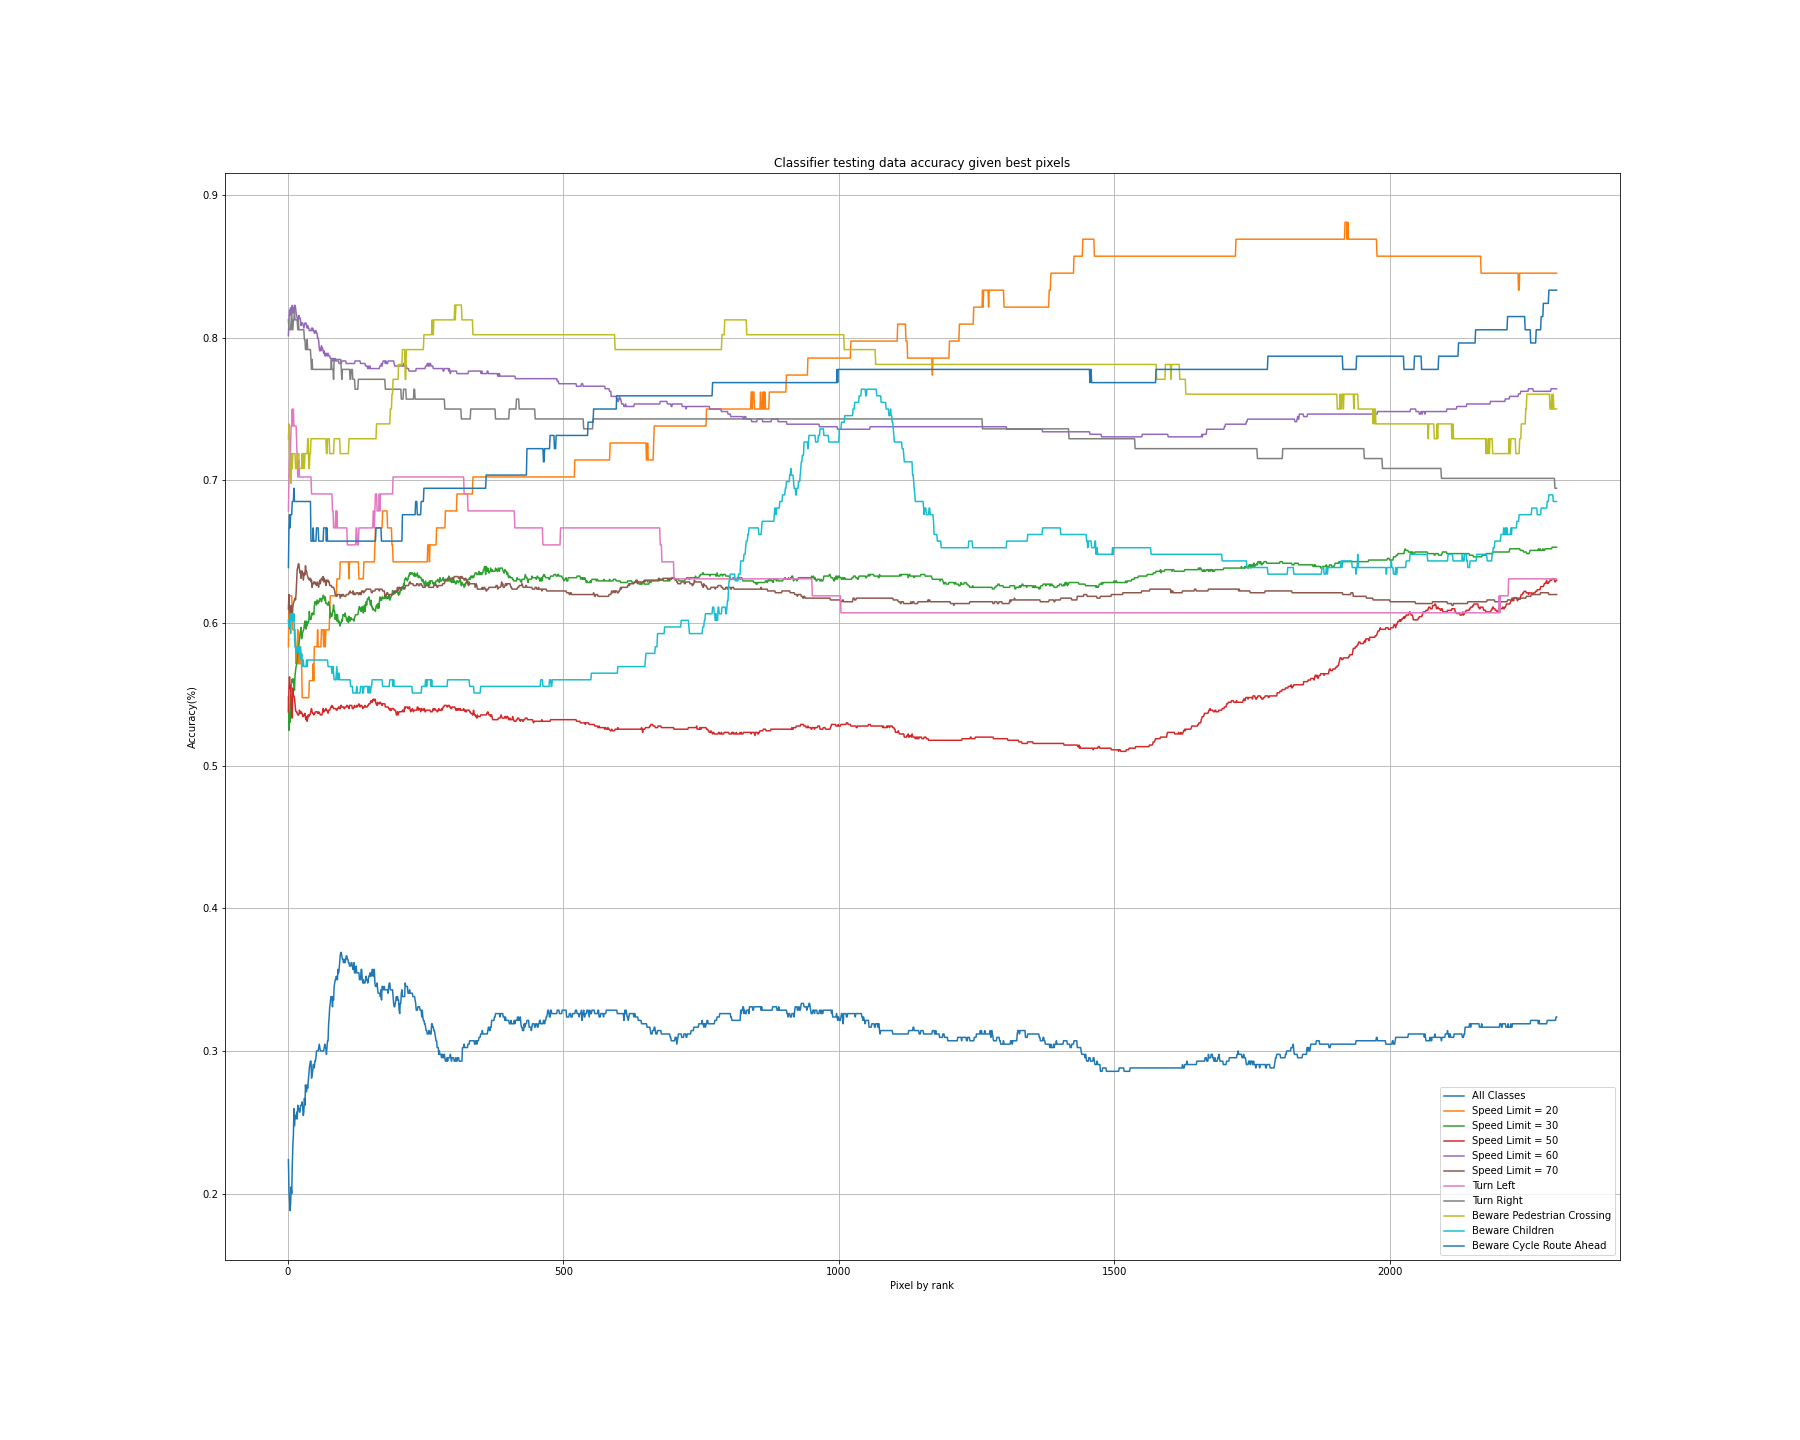
\includegraphics[width=0.95\textwidth]{Images/test_2304_pixels.png}
\end{figure}

\newpage
\subsection{Accuracy of Equal Width Binning on Train data}\label{BarChartEWBTrain}
\begin{figure}[h!]
  \centering
  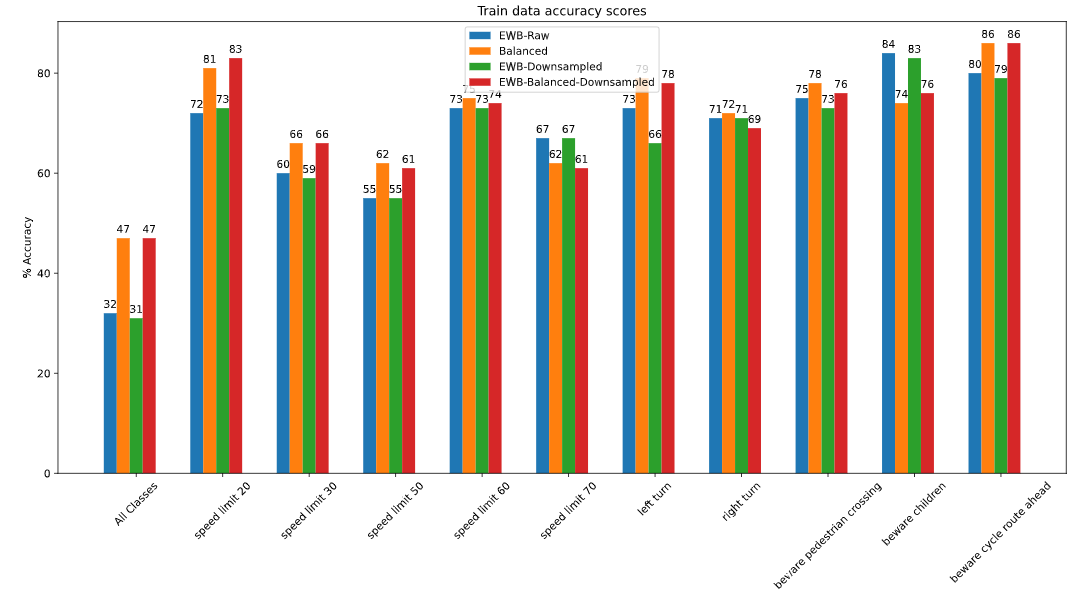
\includegraphics[width=1\textwidth]{Images/BarChartEWBTrain.PNG}
\end{figure}

\subsection{Accuracy of Equal Width Binning on Test data}\label{BarChartEWBTest}
  \begin{figure}[h!] 
    \centering
    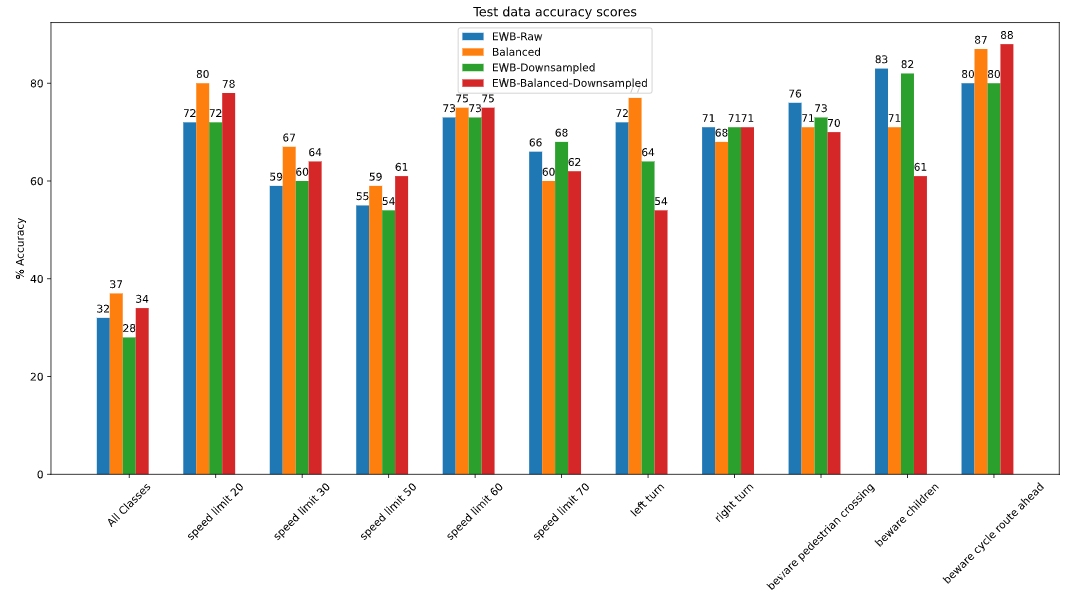
\includegraphics[scale=0.6]{images/BarChartEWBTest.PNG}
\end{figure}

\newpage
\subsection{Training confusion matrices for Naive Bayes}\label{NaiveBayesConfMatTraining}
\begin{figure}[h!]
  \centering
  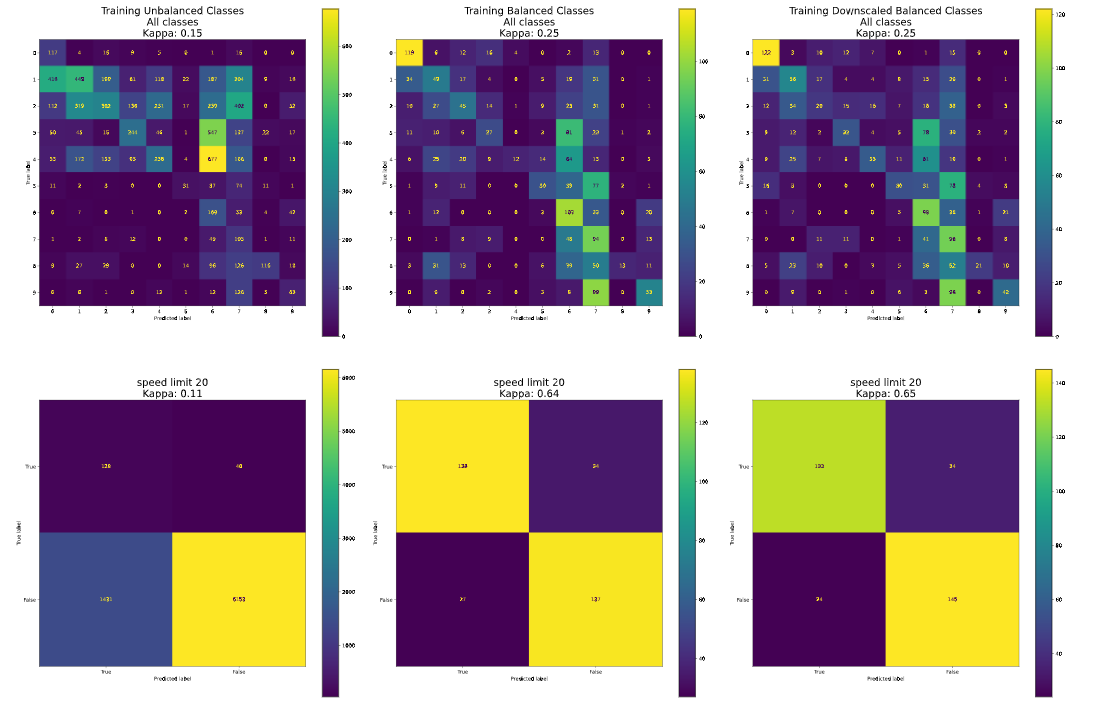
\includegraphics[width=1\textwidth]{Images/NaiveBayesConfMatTraining.PNG}
\end{figure}

\newpage
\subsection{No clusters of classes}\label{app:BadClustering}
\begin{figure}[h!]
    \centering
    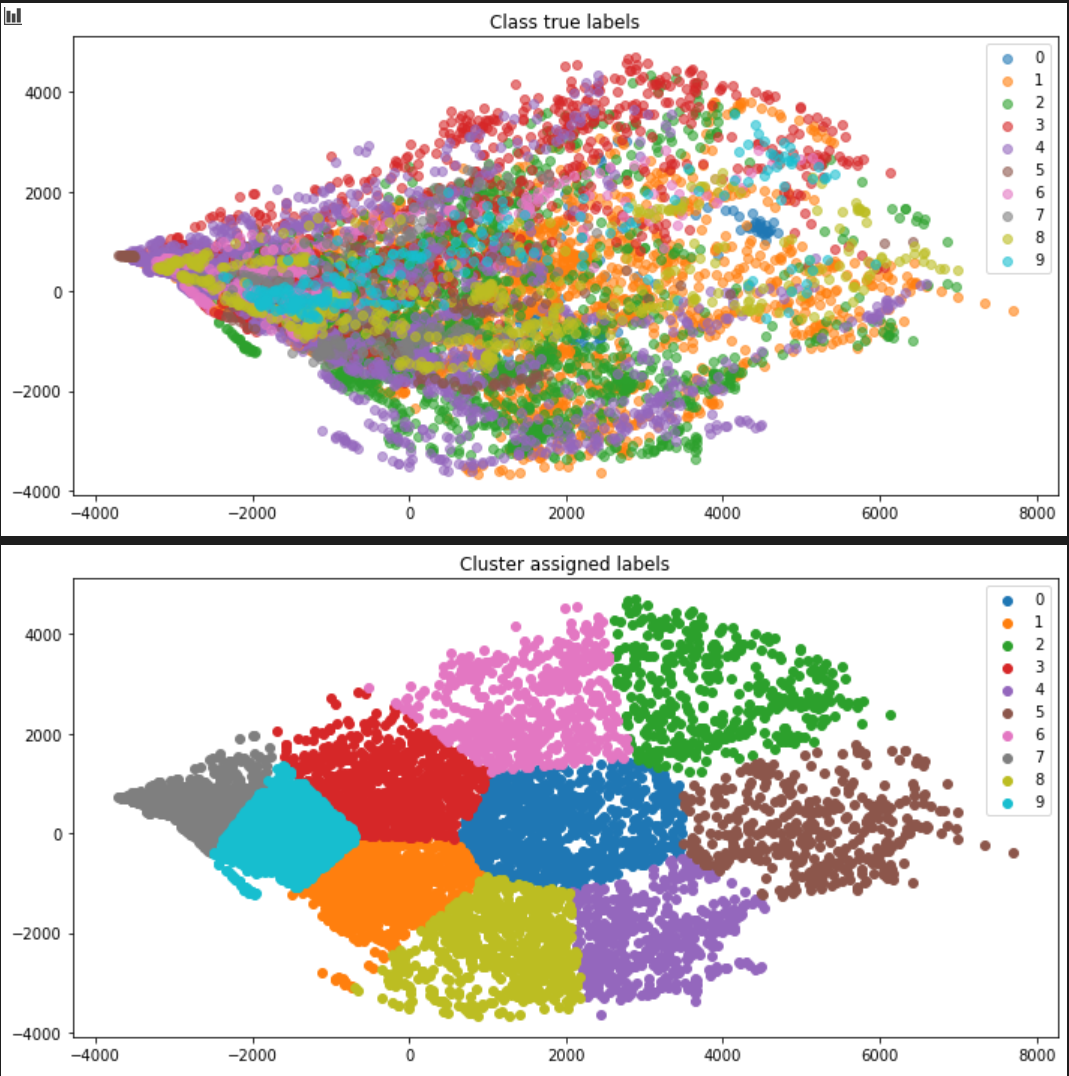
\includegraphics[width=0.95\textwidth]{Images/BadClustering.png}
\end{figure}

\newpage
\subsection{Averaged by Column Downsampled vs Average by Row Downsampled}\label{AvColDSvAvRowDS}
\begin{figure}[h!]
  \centering
  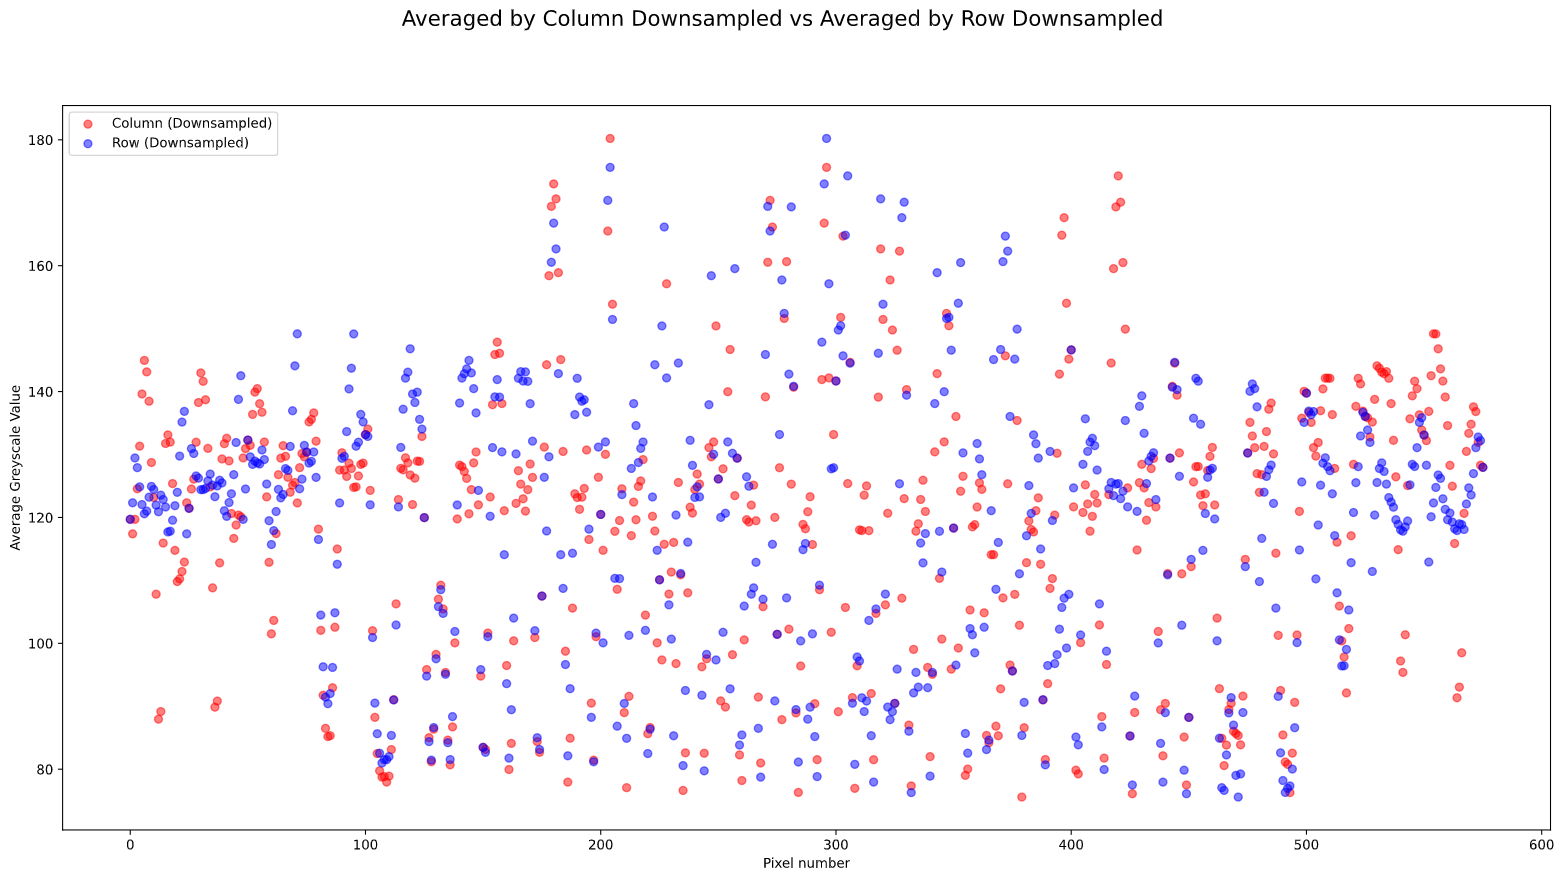
\includegraphics[width=0.95\textwidth]{Images/AvColDS vs AvRowDS.png}
\end{figure}

\subsection{12x12 Downsampled image}\label{12x12Scatter} 
\begin{figure}[h!]
  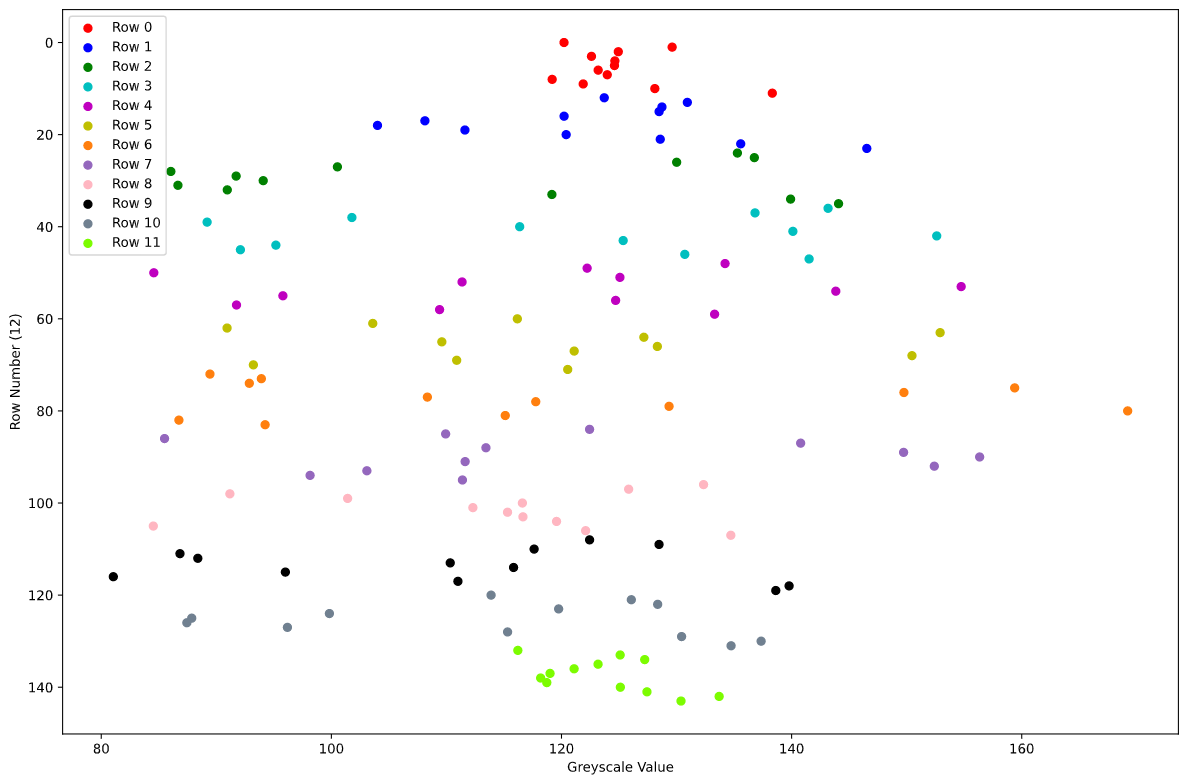
\includegraphics[width=0.85\textwidth]{Images/12x12 Scatter.png}
\end{figure}

\newpage
\subsection{Triangular and Circular sign clusters}\label{TrianCircCluster1} 
\begin{figure}[h!]
  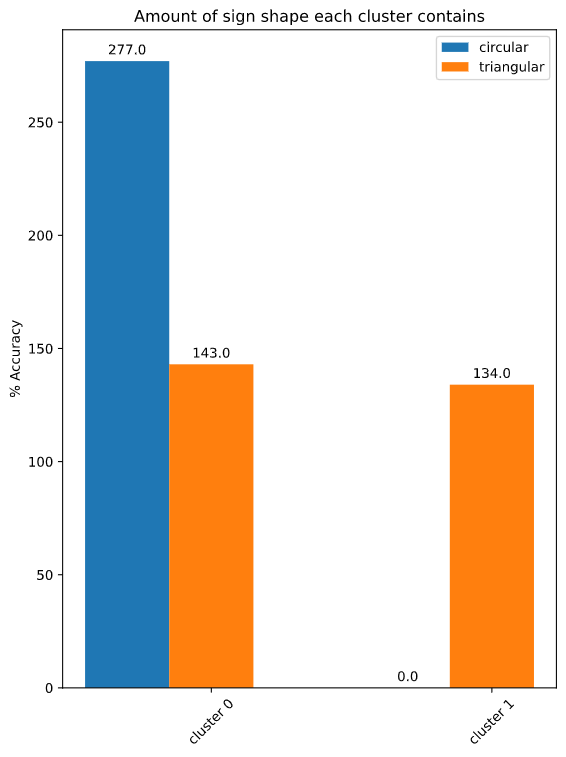
\includegraphics[width=0.85\textwidth]{Images/TriangularCircularClusterBarChart.png}
\end{figure}

\newpage
\subsection{Triangular and Circular sign clusters}\label{TrianCircCluster2} 
\begin{figure}[h!]
  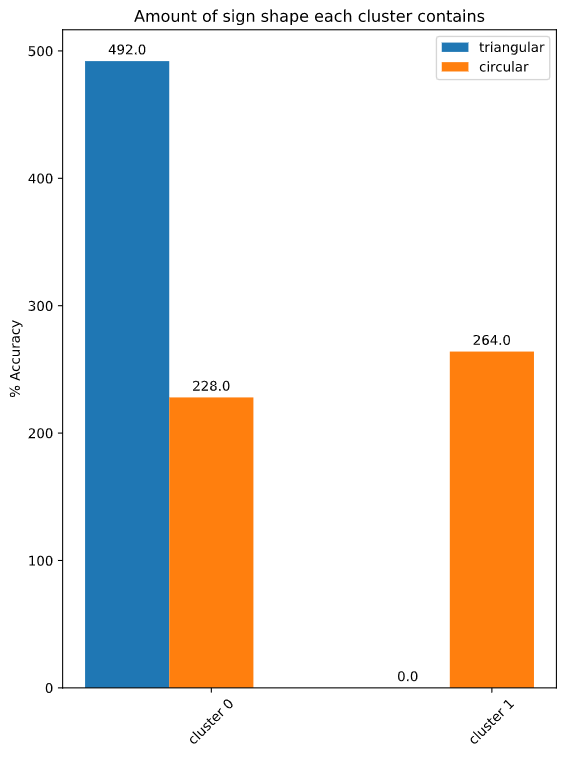
\includegraphics[width=0.85\textwidth]{Images/TriangularCircularClusterBarChart2.png}
\end{figure}

\newpage
\subsection{Test data comparison with 500 pixels}\label{500pixelsTestdata}
\begin{figure}[h!]
  \centering
  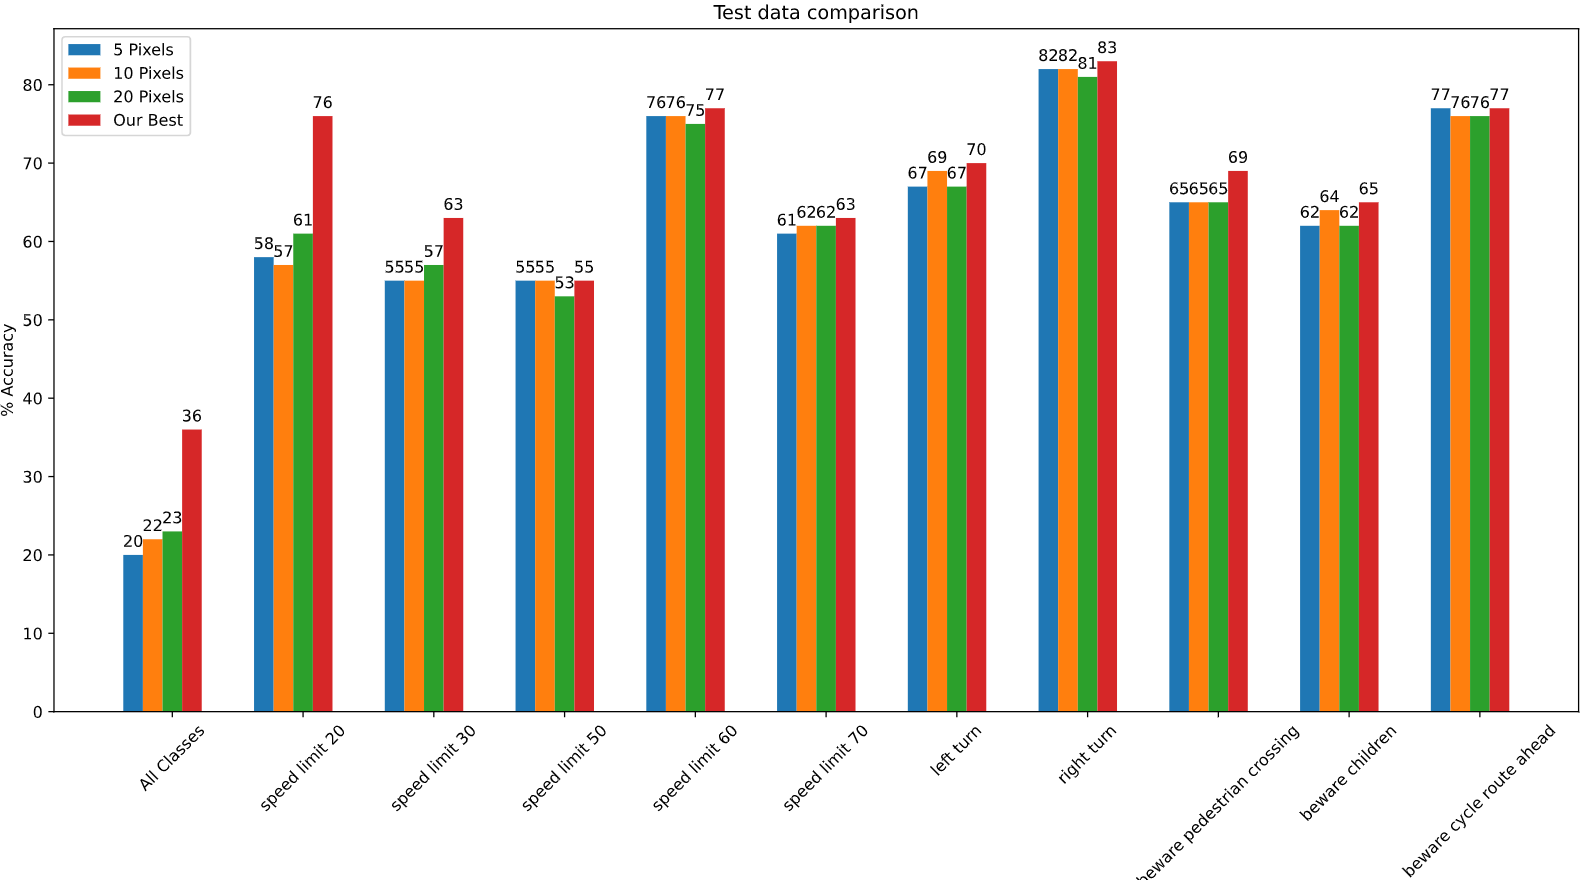
\includegraphics[scale=0.4]{images/test_data_500_pixels.PNG}
\end{figure}

\newpage
\subsection{Train data comparison with 500 pixels}\label{test_data_500_pixels}
\begin{figure}[h!]
  \centering
  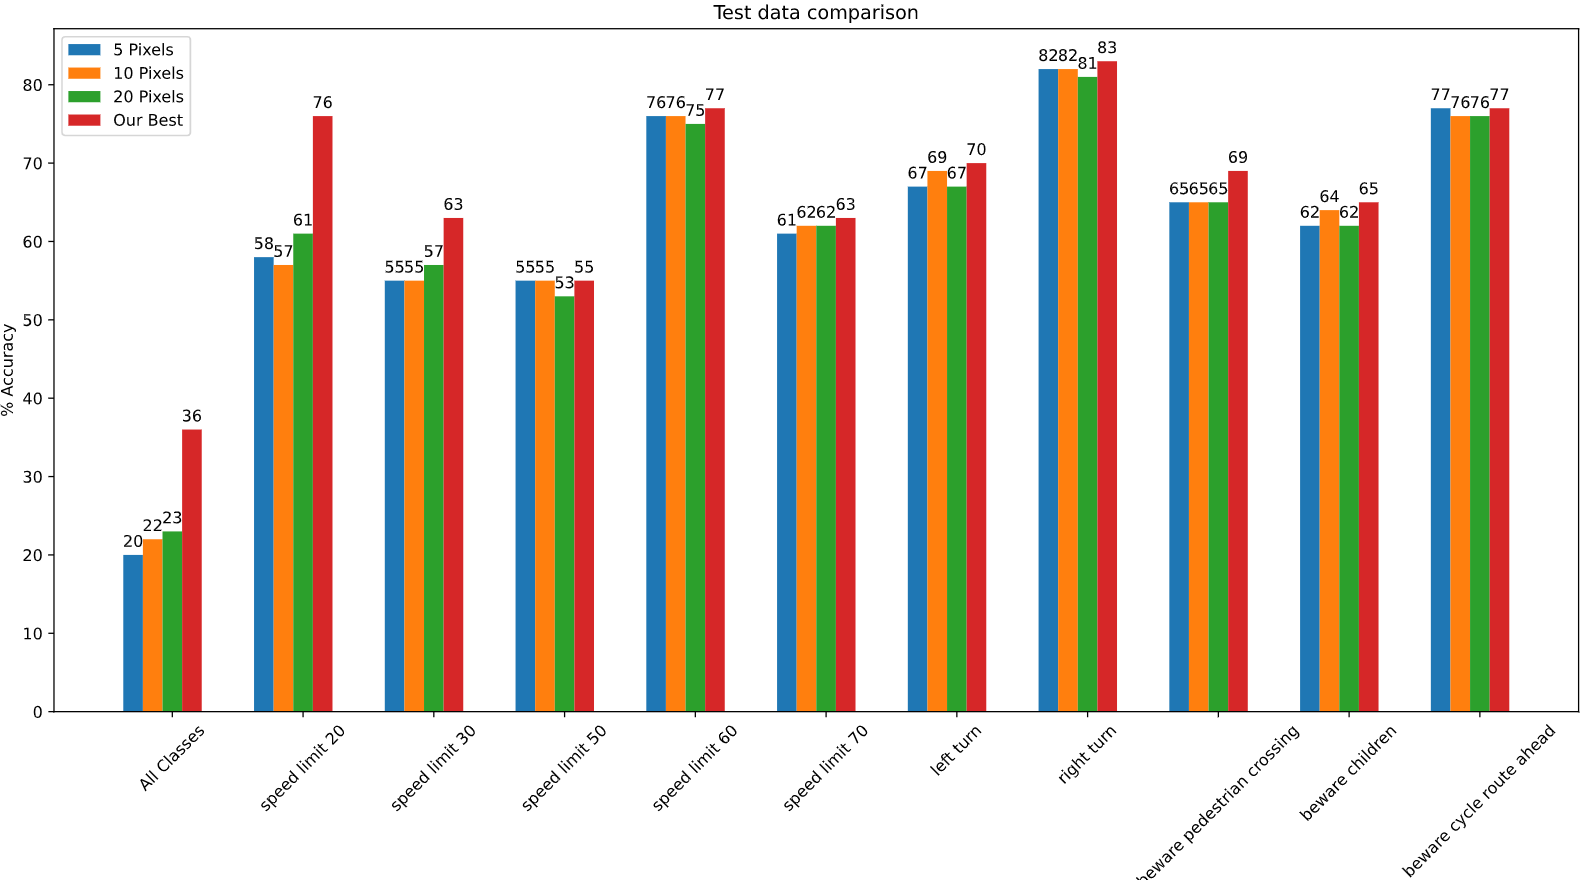
\includegraphics[scale=0.4]{images/test_data_500_pixels.PNG}
\end{figure}

\newpage
\subsection{Clustering Labels}\label{LabelClusters1} 
\begin{figure}[h!]
  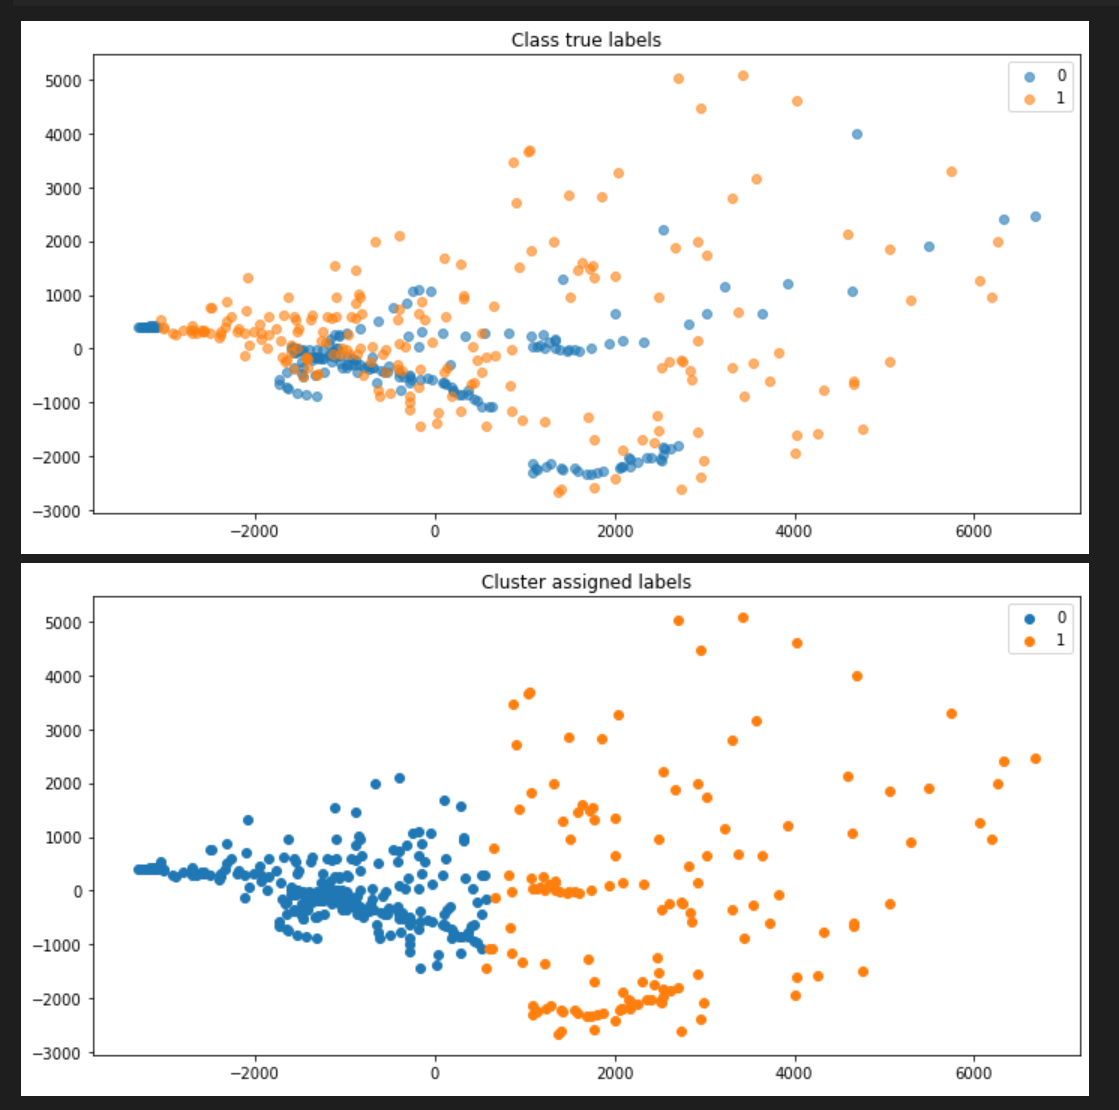
\includegraphics[width=0.8\textwidth]{Images/LabelClusters1.png}
\end{figure}

\newpage
\subsection{Clustering Labels 250 best pixels}\label{LabelClusters2} 
\begin{figure}[h!]
  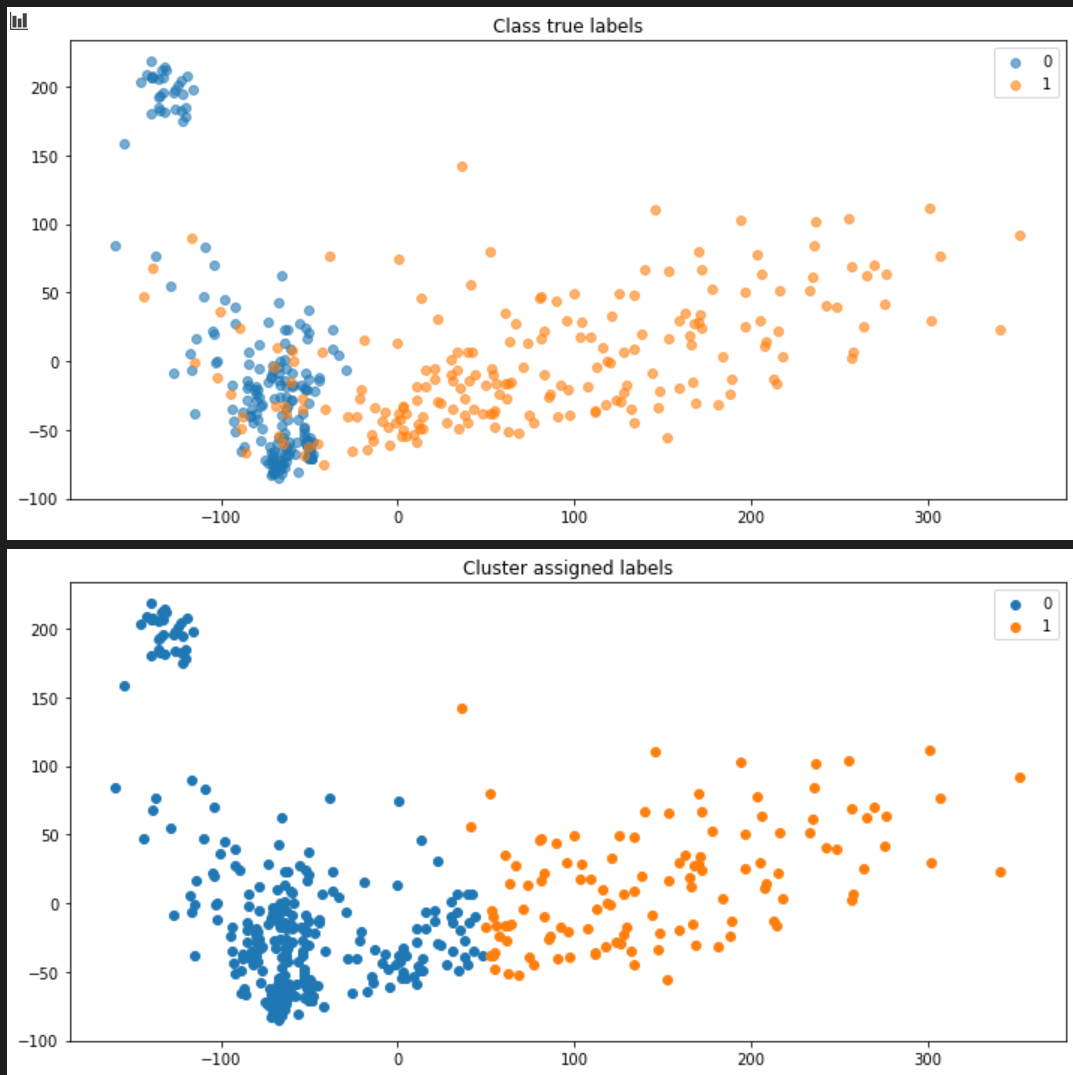
\includegraphics[width=0.8\textwidth]{Images/LabelClusters2.png}
\end{figure}

\newpage
\subsection{Networks by class}\label{ClassNetworks} 
\begin{figure}[h!]
  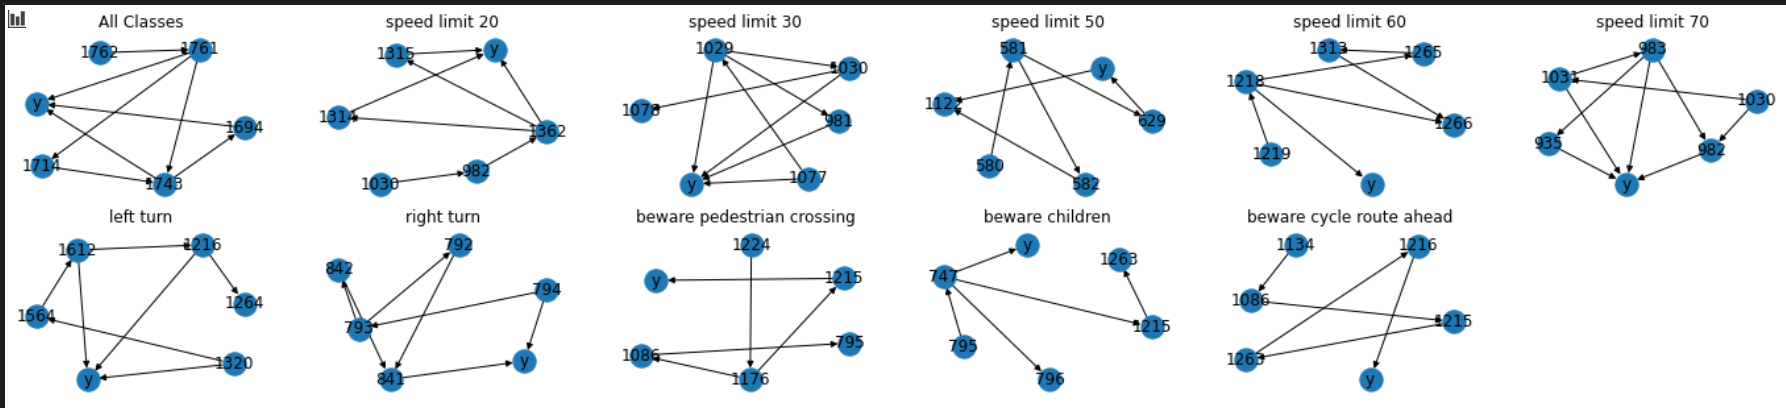
\includegraphics[width=0.85\textwidth]{Images/AllClasses.png}
\end{figure}

\end{appendices}
\end{document}
